\chapter{氧化与还原}\label{ch:g11:redox}

一条锌片浸入蓝色的硫酸铜溶液中。几
分钟内，锌片表面变暗，覆上一层海绵状的红棕色物质；一小时
后，溶液的蓝色褪去。出现了铜单质
原先没有铜的地方，锌则以看不见的离子形式进入溶液。
没有加热，没有放出气体，也没有氧气参与——然而
化学家仍把它称为氧化。这个词原指“与氧结合”
，如今它的含义更为广泛、更为实用：
即失去电子。本章将跟随电子的去向。

\begin{recall}
离子是指获得或失去电子的原子或原子团
（见\cref{ch:g9:ions}）。铁、锌等金属与
盐酸反应，生成氢气和金属离子
（见\cref{ch:g9:metals-acids-corrosion}）。物质的量 $n$，以摩尔为单位，
可由质量 $m$ 按 $n = m/M$ 算出，
（见\cref{ch:g10:the-mole}）。
\end{recall}

\begin{omfigure}
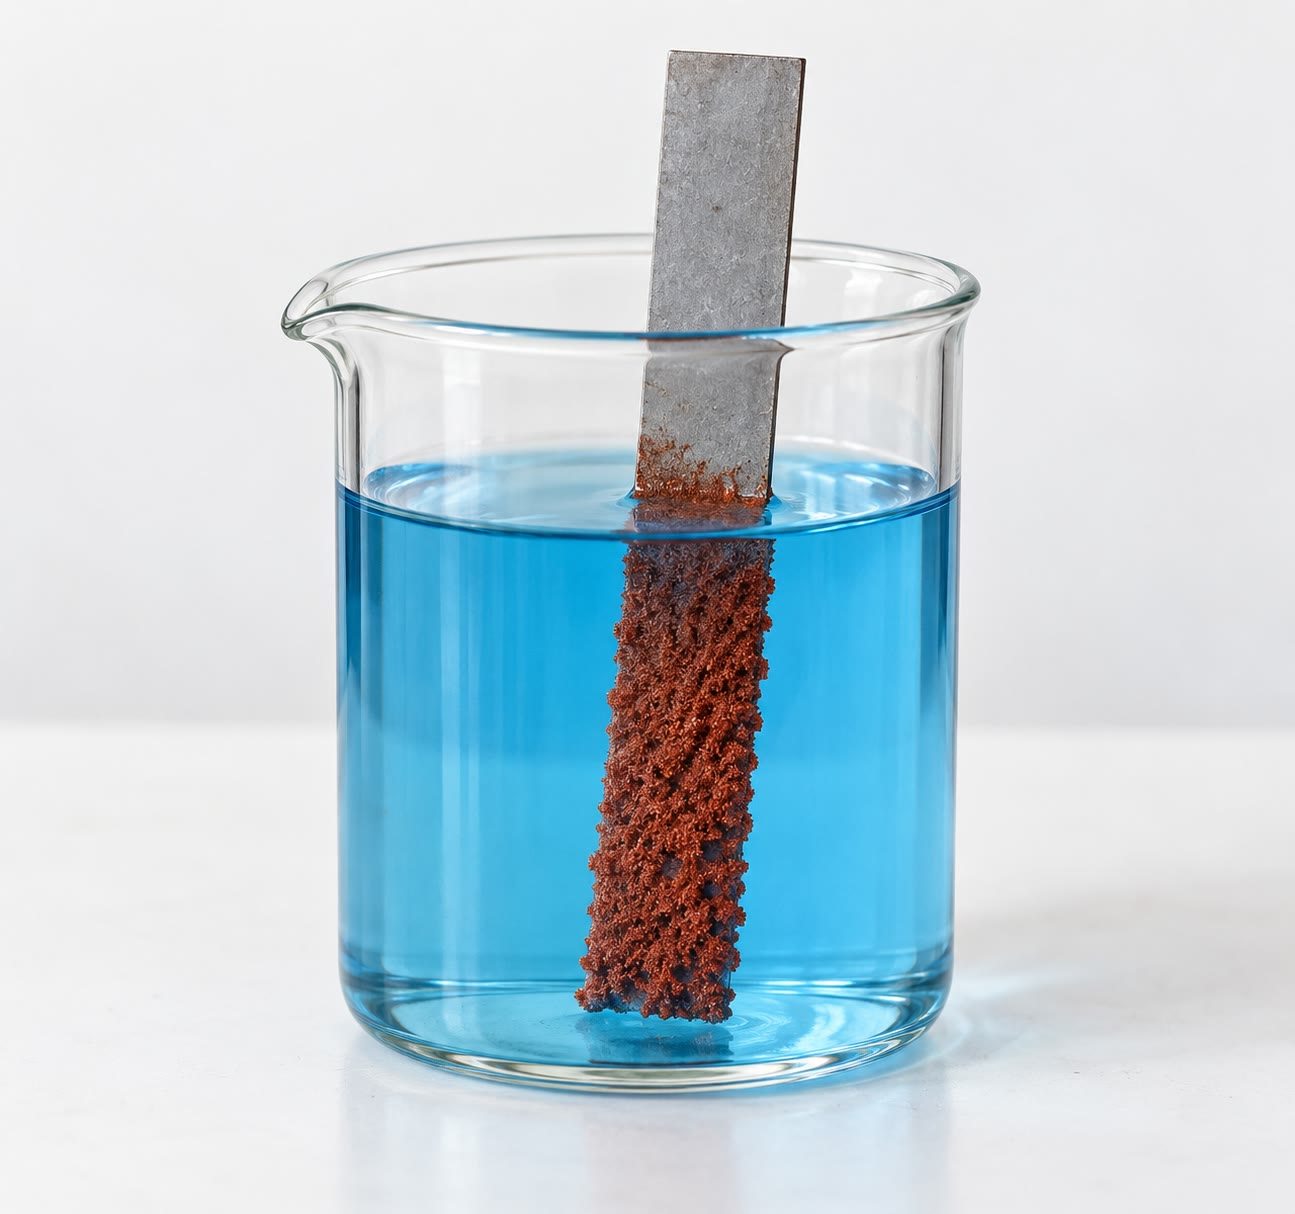
\includegraphics[width=0.55\linewidth]{images/book1/ai/g11-zinc-copper-sulfate.jpg}

{\small 锌片置于硫酸铜溶液中：铜沉积在
锌片上，锌离子则进入溶液。}
\end{omfigure}

\section{氧化剂与还原剂}

\begin{definition}[氧化剂与还原剂]\label{def:g11:redox:oxidant}
能够得到一个或多个电子的粒子称为\emph{氧化剂}\index{氧化剂}，
能够失去一个或多个电子的粒子称为
\emph{还原剂}\index{还原剂}。
\end{definition}

\begin{definition}[氧化与还原]\label{def:g11:redox:oxidation}
\emph{氧化}\index{氧化}是失去电子；
\emph{还原}\index{还原}是得到电子。还原剂
被氧化，氧化剂被还原。
\end{definition}

\begin{remark}[记忆方法]\label{rem:g11:redox:remember}
在\emph{还原}中，粒子的电荷减小：\ce{Cu^{2+}}
得到两个电子后变为\ce{Cu}，电荷由 $+2 \to 0$。在
氧化中电荷升高：\ce{Zn -> Zn^{2+} + 2e-}，$0 \to +2$。
\end{remark}

\begin{definition}[氧化还原电对与半反应式]\label{def:g11:redox:couple}
氧化剂及其得到电子后所成的还原剂构成一个
\emph{氧化还原电对}\index{氧化还原电对}，记作 Ox/Red，氧化剂居前：
如 \ce{Cu^{2+}}/\ce{Cu}、\ce{Zn^{2+}}/\ce{Zn}。电对内的电子交换
可用其
\emph{半反应式}\index{半反应式}，
\[
  \text{Ox} + n\,\ce{e-} \ce{<=>} \text{Red}, % ce-unbalanced-ok (generic form)
\]
原子和电荷都已配平，例如
$\ce{Cu^{2+}(aq) + 2e- <=> Cu(s)}$。双箭头表示
该交换可朝两个方向进行。
\end{definition}

\begin{example}[金属及其离子]\label{ex:g11:redox:metals}
每种金属都与其离子构成一个电对：
\begin{center}
\begin{tabular}{ll}
\hline
电对 & 半反应式 \\
\hline
\ce{Ag+}/\ce{Ag} & \ce{Ag+ + e- <=> Ag} \\
\ce{Cu^{2+}}/\ce{Cu} & \ce{Cu^{2+} + 2e- <=> Cu} \\
\ce{Fe^{2+}}/\ce{Fe} & \ce{Fe^{2+} + 2e- <=> Fe} \\
\ce{Zn^{2+}}/\ce{Zn} & \ce{Zn^{2+} + 2e- <=> Zn} \\
\ce{Al^{3+}}/\ce{Al} & \ce{Al^{3+} + 3e- <=> Al} \\
\hline
\end{tabular}
\end{center}
离子也能构成电对：\ce{Fe^{3+} + e- <=> Fe^{2+}} 对应电对
\ce{Fe^{3+}}/\ce{Fe^{2+}}，\ce{I2 + 2e- <=> 2I-} 对应
电对 \ce{I2}/\ce{I-}。氢也是如此：\ce{2H+ + 2e- <=> H2} 对应
电对 \ce{H+}/\ce{H2}。
\end{example}

\begin{remark}[一个粒子，两种角色]\label{rem:g11:redox:amphoteric}
同一粒子既可以是一个电对的还原剂，也可以是另一电对的氧化剂。
例如离子 \ce{Fe^{2+}} 是 \ce{Fe^{2+}}/\ce{Fe} 的氧化剂，同时
是 \ce{Fe^{3+}}/\ce{Fe^{2+}} 的还原剂。它扮演哪种角色，
取决于反应中与它配对的物质。
\end{remark}

\section{氧化还原反应}

\begin{definition}[氧化还原反应]\label{def:g11:redox:reaction}
\emph{氧化还原反应}\index{氧化还原反应}是电子从
一个电对的还原剂转移到另一电对的氧化剂。
还原剂被氧化，氧化剂被还原，两者同时进行。
\end{definition}

\begin{proposition}[不存在自由电子]\label{prop:g11:redox:no-free-electrons}
溶液中的电子不能单独存在：还原剂给出的每个电子
都会被氧化剂接受。因此，氧化还原反应的方程式
可由两个半反应式各乘以适当的系数后相加得到，
这些系数应使失去的电子数与得到的电子数相等；
电子随即相互抵消，不出现在方程式中。
\end{proposition}

\begin{example}[锌与铜离子]\label{ex:g11:redox:zinc-copper}
在开头的情境中，锌被氧化，铜离子
被还原：
\[
\begin{array}{l@{\qquad}l}
  \ce{Zn(s) -> Zn^{2+}(aq) + 2e-} & \text{（氧化）}\\
  \ce{Cu^{2+}(aq) + 2e- -> Cu(s)} & \text{（还原）}\\
  \hline
  \ce{Zn(s) + Cu^{2+}(aq) -> Zn^{2+}(aq) + Cu(s)} &
\end{array}
\]
每个锌原子向一个铜离子转移两个电子。溶液的蓝色
正是 \ce{Cu^{2+}} 离子的颜色；随着它们被消耗，
蓝色逐渐褪去，无色的 \ce{Zn^{2+}} 离子
则取而代之。
\end{example}

\begin{omfigure}
\begin{tikzpicture}[font=\small, >=Stealth,
    ion/.style={circle, draw=black!70, minimum size=10mm, inner sep=0pt}]
  % the zinc strip and the solution
  \fill[black!18] (0,0) rectangle (1.6,4);
  \draw[black!60] (1.6,0) -- (1.6,4);
  \node[anchor=south] at (0.8,0.08) {锌};
  \fill[omWater!60] (1.6,0) rectangle (9.0,4);
  \node[anchor=north east] at (8.95,3.95) {溶液};
  % a zinc atom leaves as an ion
  \node[ion, fill=black!30] (zn) at (1.15,3.0) {\ce{Zn}};
  \node[ion, fill=white] (znion) at (5.0,3.0) {\ce{Zn^{2+}}};
  \draw[->, thick, omProp] (zn.east) -- (znion.west)
    node[midway, above] {氧化};
  % the electrons travel through the metal
  \draw[->, thick, omDef, dashed] (0.75,2.45) -- (0.75,1.55)
    node[midway, right] {2\,\ce{e-}};
  % a copper ion is reduced on the surface
  \node[ion, fill=omDef!35] (cuion) at (5.0,1.0) {\ce{Cu^{2+}}};
  \node[ion, fill=orange!55!brown] (cu) at (2.12,1.0) {\ce{Cu}};
  \draw[->, thick, omProp] (cuion.west) -- (cu.east)
    node[midway, above] {还原};
  \node[anchor=west, align=left] at (6.1,2.0) {每个锌原子给出 \\ 两个电子给一个 \\ 铜离子};
\end{tikzpicture}

{\small 在锌的表面。一个锌原子失去两个电子，
以 \ce{Zn^{2+}} 离子的形式离开，两个电子
经金属流向与表面接触的 \ce{Cu^{2+}} 离子，
该离子变成铜原子，留在金属片上。}
\end{omfigure}

\begin{omfigure}
\begin{tikzpicture}[font=\small]
  \pic at (0,0) {beaker={0.75}{omDef!45}};
  \fill[black!35] (-0.15,0.25) rectangle (0.15,2.5);
  \draw[black!65] (-0.15,0.25) rectangle (0.15,2.5);
  \node[anchor=north, align=center] at (0,-0.15) {开始时：\\ 蓝色的 \ce{Cu^{2+}} 溶液};
  \draw[->, thick, omProp] (1.3,1) -- (3.2,1) node[midway, above] {一小时};
  \pic at (4.5,0) {beaker={0.75}{omDef!12}};
  \fill[black!35] (4.35,0.25) rectangle (4.65,2.5);
  \fill[orange!55!brown] (4.3,0.25) rectangle (4.7,1.5);
  \draw[black!65] (4.35,0.25) rectangle (4.65,2.5);
  \node[anchor=north, align=center] at (4.5,-0.15) {之后：溶液颜色变浅，\\ 锌片上有铜};
\end{tikzpicture}

{\small 可以观察到：浸入溶液中的锌片部分上有铜沉积，
以及 \ce{Cu^{2+}} 离子蓝色的褪去。}
\end{omfigure}

\begin{example}[酸中的金属再探]\label{ex:g11:redox:acid}
铁溶解于盐酸中时，铁被氧化，
而 \ce{H+} 离子被还原为氢气：
\[
  \ce{Fe(s) + 2H+(aq) -> Fe^{2+}(aq) + H2(g)}.
\]
电对为 \ce{Fe^{2+}}/\ce{Fe} 和 \ce{H+}/\ce{H2}；氯
离子不参与反应。
\end{example}

\begin{inthelab}[银树]
将一圈洁净的铜丝悬挂于盛有稀硝酸银溶液的烧杯中，
即 \ce{Ag+(aq) + NO3^-(aq)}。一小时内，树枝状的
光亮的银沿铜丝生长，无色溶液变为
淡蓝色：\ce{Cu(s) + 2Ag+(aq) -> Cu^{2+}(aq) + 2Ag(s)}。
实验由教师操作，需戴手套和护目镜，而
溶液事后作为危险废物收集。
\end{inthelab}

\begin{safety}{\ghs[0.82cm]{GHS03}\ghs[0.82cm]{GHS05}\ghs[0.82cm]{GHS08}\ghs[0.82cm]{GHS09}}
% ledger: ghs:AgNO3
硝酸银：能助燃的氧化剂（GHS03）；对皮肤和
眼睛有腐蚀性，会使皮肤染黑（GHS05）；对健康有害
（GHS08）；对水生生物剧毒，因此决不可倒入
水槽（GHS09）。
\end{safety}

\begin{omfigure}
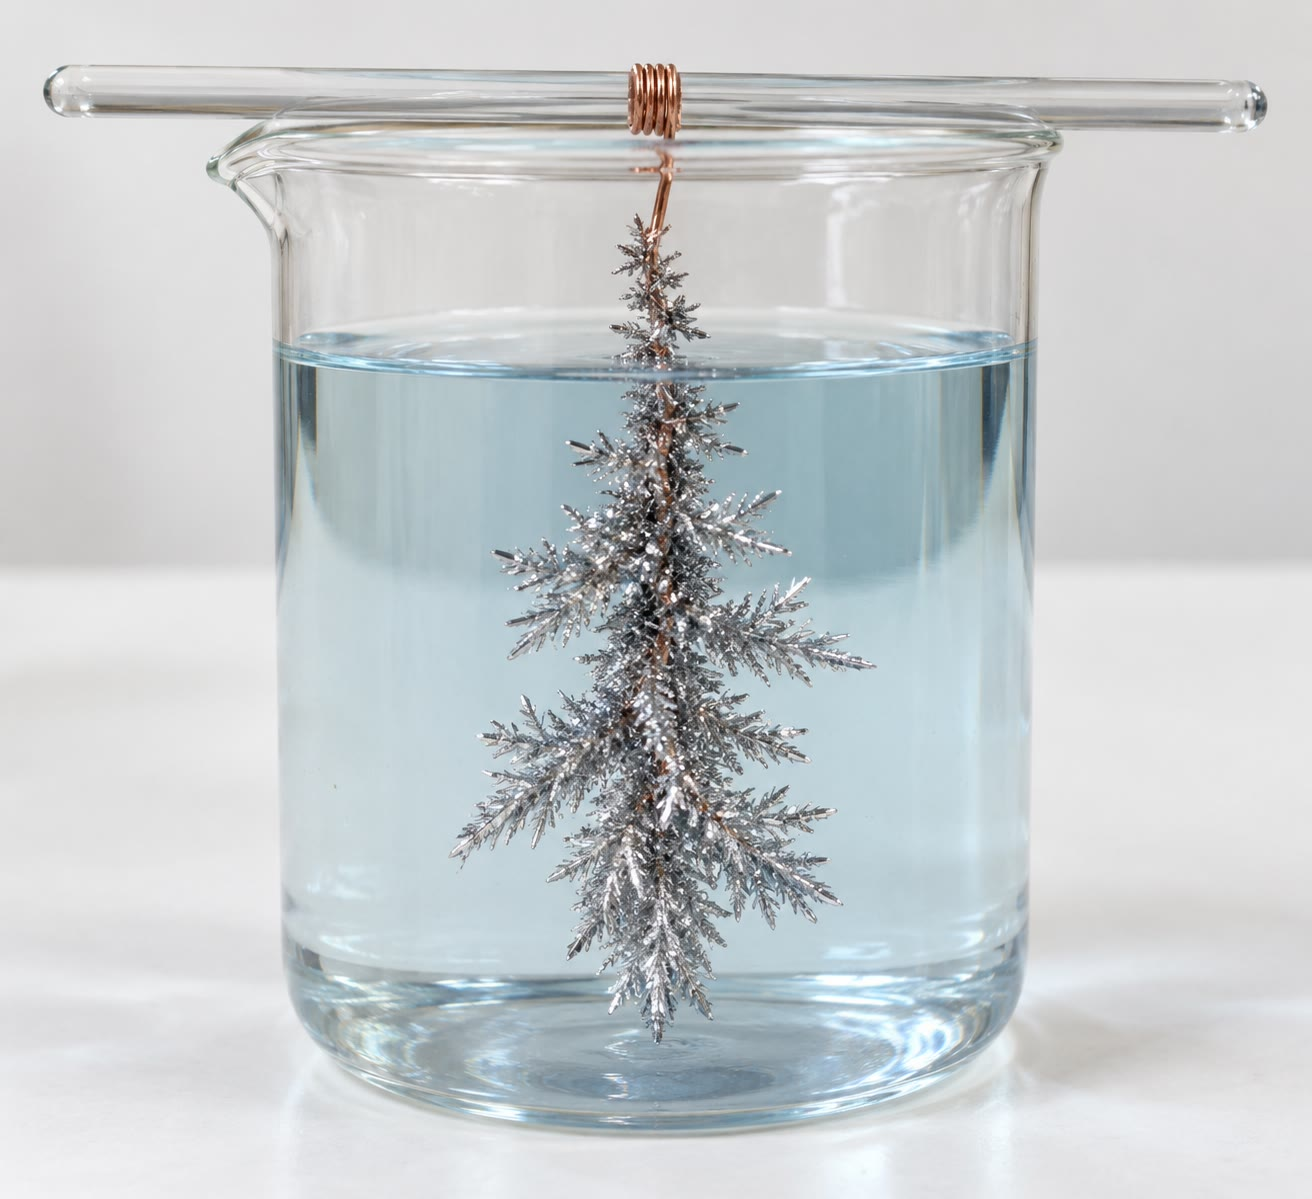
\includegraphics[width=0.5\linewidth]{images/book1/ai/g11-silver-tree.jpg}

{\small 银晶体在铜丝上生长，
位于硝酸银溶液中。}
\end{omfigure}

\section{配平半反应式}

许多重要的电对含有氧，且是针对酸性
溶液书写的，其中存在 \ce{H+} 离子。其半反应式
需用水分子和 \ce{H+} 离子来配平。

\begin{method}[酸性溶液中配平半反应式]\label{met:g11:redox:balance}
在酸性溶液中写出电对 Ox/Red 的半反应式：
\begin{enumerate}
  \item 将 Ox 写在左侧、Red 写在右侧，配平
        既非 O 也非 H 的原子；
  \item 用水分子 \ce{H2O} 配平氧原子；
  \item 用 \ce{H+} 离子配平氢原子；
  \item 在左侧用电子 \ce{e-} 配平电荷；
  \item 检查：两边各原子数目相同，两侧
        总电荷相同。
\end{enumerate}
\end{method}

\begin{example}[高锰酸根离子]\label{ex:g11:redox:permanganate}
对于电对 \ce{MnO4^-}/\ce{Mn^{2+}}（深紫色变为几乎
无色）：锰已配平；左侧 4 个氧原子给出右侧
的 $\ce{4H2O}$；8 个氢原子给出左侧的 $\ce{8H+}$；
左侧电荷为 $-1 + 8 = +7$，右侧为 $+2$，故
左侧需加入 5 个电子：
\[
  \ce{MnO4^-(aq) + 8H+(aq) + 5e- <=> Mn^{2+}(aq) + 4H2O(l)}.
\]
\end{example}

\begin{example}[重铬酸根离子]\label{ex:g11:redox:dichromate}
对于电对 \ce{Cr2O7^{2-}}/\ce{Cr^{3+}}（橙色变为绿色）：右侧有 2 个铬原子；
7 个氧原子给出 \ce{7H2O}；14 个氢原子给出 \ce{14H+}；电荷
左侧为 $-2 + 14 = +12$，右侧为 $2 \times 3 = +6$，故
左侧需加入 6 个电子：
\[
  \ce{Cr2O7^{2-}(aq) + 14H+(aq) + 6e- <=> 2Cr^{3+}(aq) + 7H2O(l)}.
\]
\end{example}

\begin{method}[写出氧化还原方程式]\label{met:g11:redox:combine}
写出一个电对的氧化剂 Ox$_1$ 与
另一电对的还原剂 Red$_2$ 之间反应的方程式：
\begin{enumerate}
  \item 分别写出两个半反应式：第一个按还原方向
        （Ox$_1 \to$ Red$_1$），第二个按氧化方向
        （Red$_2 \to$ Ox$_2$）；
  \item 将两式各乘以使电子数相等的
        最小整数；
  \item 两式相加，电子相消，两边都出现的 \ce{H+} 和
        \ce{H2O} 也可能相消；
  \item 再次检查原子和电荷是否守恒。
\end{enumerate}
\end{method}

\begin{example}[高锰酸根与铁（II）]\label{ex:g11:redox:mno4-fe}
高锰酸根离子将 \ce{Fe^{2+}} 氧化为 \ce{Fe^{3+}}：
\[
\begin{array}{l@{\qquad}l}
  \ce{MnO4^- + 8H+ + 5e- -> Mn^{2+} + 4H2O} & \times 1\\
  \ce{Fe^{2+} -> Fe^{3+} + e-} & \times 5\\
  \hline
  \ce{MnO4^- + 8H+ + 5Fe^{2+} -> Mn^{2+} + 5Fe^{3+} + 4H2O} &
\end{array}
\]
左侧电荷为 $-1 + 8 + 10 = +17$；右侧为 $2 + 15 = +17$。
这一反应在下一章中用于测定
铁（II）的物质的量。
\end{example}

\section{生活中的氧化剂与还原剂}

\begin{proposition}[一些常见的氧化剂与还原剂]\label{prop:g11:redox:common}
下列物质在实验室中反复出现，
在日常生活中也十分常见：
\begin{center}
\small
\begin{tabular}{lll}
\hline
物质 & 作用 & 其电对的半反应式 \\
\hline
氧气 \ce{O2} & 氧化剂 & \ce{O2 + 4H+ + 4e- <=> 2H2O} \\
氯气 \ce{Cl2} & 氧化剂 & \ce{Cl2 + 2e- <=> 2Cl-} \\
次氯酸根 \ce{ClO-}（漂白剂） & 氧化剂 & \ce{2ClO- + 4H+ + 2e- <=> Cl2 + 2H2O} \\
过氧化氢 \ce{H2O2} & 氧化剂 & \ce{H2O2 + 2H+ + 2e- <=> 2H2O} \\
高锰酸根 \ce{MnO4^-} & 氧化剂 & \ce{MnO4^- + 8H+ + 5e- <=> Mn^{2+} + 4H2O} \\
金属 \ce{M}（\ce{Fe}、\ce{Zn}、\ce{Al}\dots） & 还原剂 & \ce{M^{n+} + $n$ e- <=> M} % ce-unbalanced-ok (generic)
\\
碘离子 \ce{I-} & 还原剂 & \ce{I2 + 2e- <=> 2I-} \\
硫代硫酸根 \ce{S2O3^{2-}} & 还原剂 & \ce{S4O6^{2-} + 2e- <=> 2S2O3^{2-}} \\
抗坏血酸 \ce{C6H8O6}（维生素 C） & 还原剂 & \ce{C6H6O6 + 2H+ + 2e- <=> C6H8O6} \\
\hline
\end{tabular}
\end{center}
\end{proposition}

\begin{example}[铜变绿]\label{ex:g11:redox:patina}
铜制屋顶和铜像长期暴露在空气中，
缓慢变为淡绿色。空气中的氧将铜氧化为 \ce{Cu^{2+}} 离子，
这些离子与水和二氧化碳结合，形成一层薄薄的绿色锈层，即铜绿。
与铁锈不同，铜绿附着在金属表面，
并能保护金属免受进一步的侵蚀。
\end{example}

\begin{omfigure}

\includegraphics[width=0.48\linewidth]{images/book1/ai/g11-green-roof.jpg}

{\small 空气中放置数十年的铜制屋顶：被氧化的铜形成
绿色的铜绿。}
\end{omfigure}

\begin{remark}[抗氧化剂]\label{rem:g11:redox:antioxidant}
加入食物中的“抗氧化剂”是一种还原剂，它会先于食物被
空气中的氧氧化。维生素 C（抗坏血酸）是最常见的
例子：撒上柠檬汁的切开苹果，褐变要慢得多，
因为柠檬中的维生素 C 先被氧化。
\end{remark}

\section{练习}

\begin{exercise}[$\star$]\label{exo:g11:redox:1}
定义氧化剂、还原剂、氧化和还原。
\end{exercise}

\begin{exercise}[$\star$]\label{exo:g11:redox:2}
对每一对物质，将氧化还原电对写成 Ox/Red 的形式：\ce{Fe} 与
\ce{Fe^{2+}}；\ce{Ag} 与 \ce{Ag+}；\ce{I-} 与 \ce{I2}；\ce{Fe^{2+}}
与 \ce{Fe^{3+}}。
\end{exercise}

\begin{exercise}[$\star$]\label{exo:g11:redox:3}
写出下列电对的半反应式：\ce{Ag+}/\ce{Ag}、
\ce{Al^{3+}}/\ce{Al}、\ce{Fe^{3+}}/\ce{Fe^{2+}} 和 \ce{Cl2}/\ce{Cl-}。
\end{exercise}

\begin{exercise}[$\star$]\label{exo:g11:redox:4}
转化 \ce{Fe -> Fe^{2+} + 2e-} 是氧化还是
还原？铁在其中是作氧化剂还是还原剂？
\end{exercise}

\begin{exercise}[$\star$]\label{exo:g11:redox:5}
在反应 \ce{Zn + Cu^{2+} -> Zn^{2+} + Cu} 中，指出
被氧化的物质、被还原的物质、氧化剂和还原剂，
并给出每个锌原子转移的电子数。
\end{exercise}

\begin{exercise}[$\star\star$]\label{exo:g11:redox:6}
在酸性溶液中配平电对 \ce{H2O2}/\ce{H2O} 的半反应式，
按照\cref{met:g11:redox:balance}，
逐步进行。
\end{exercise}

\begin{exercise}[$\star\star$]\label{exo:g11:redox:7}
写出碘 \ce{I2} 与
硫代硫酸根离子 \ce{S2O3^{2-}} 的反应方程式，该反应
生成碘离子和连四硫酸根离子 \ce{S4O6^{2-}}。
\end{exercise}

\begin{exercise}[$\star\star$]\label{exo:g11:redox:8}
由两个半反应式写出银树反应的方程式，
并解释溶液为何变蓝。
\end{exercise}

\begin{exercise}[$\star\star$]\label{exo:g11:redox:9}
维生素 C，\ce{C6H8O6}，与碘 \ce{I2} 反应。写出
该反应的方程式，并指出哪种物质是还原剂。
\end{exercise}

\begin{exercise}[$\star\star$]\label{exo:g11:redox:10}
铝与铜(II)离子反应。写出方程式，并解释
为何两个半反应式必须分别乘以 2 和 3。
\end{exercise}

\begin{exercise}[$\star\star$]\label{exo:g11:redox:11}
过氧化氢在酸性溶液中
将铁(II)离子氧化为铁(III)离子。写出方程式。
\end{exercise}

\begin{exercise}[$\star\star\star$]\label{exo:g11:redox:12}
将一片锌片放入含过量铜(II)离子的溶液中，锌片质量减少 \qty{1.30}{g}。
问沉积出的铜的质量是多少？取
$M(\ce{Zn}) = \qty{65.4}{g/mol}$ 和 $M(\ce{Cu}) = \qty{63.5}{g/mol}$。
\end{exercise}

\begin{exercise}[$\star\star\star$]\label{exo:g11:redox:13}
写出酸性溶液中重铬酸根离子
氧化铁(II)离子的方程式。问被
\qty{0.010}{mol} 重铬酸根离子氧化的 \ce{Fe^{2+}} 的物质的量是多少？
\end{exercise}

\begin{exercise}[$\star\star\star$]\label{exo:g11:redox:14}
漂白液含有次氯酸根离子 \ce{ClO-} 和
氯离子 \ce{Cl-}。利用电对 \ce{ClO-}/\ce{Cl2} 和 \ce{Cl2}/\ce{Cl-}，
写出漂白液遇酸时发生反应的方程式，
并解释为何漂白液和酸性除垢剂的标签都警告
切勿混用。
\end{exercise}

\begin{exercise}[$\star\star\star$]\label{exo:g11:redox:15}
在锌表面的图中，电子通过金属传递，
而不是通过溶液。利用\cref{prop:g11:redox:no-free-electrons}，
解释为何铜沉积在锌片本身上，
而不在烧杯的其他地方。
\end{exercise}

\section{问题：呼气检测}

\begin{problem}[{周末问题——呼气酒精检测管的化学：
两个电对、橙色变绿色、检测管能检出的乙醇质量，
以及取代它的燃料电池}]
\label{pb:g11:redox:1}
% ledger: ghs:K2Cr2O7, breath:ratio; molar masses from tools/molar_mass.py
% (0.1-rounded weights): K2Cr2O7 294.2, C2H6O 46.0 g/mol
早期的呼气酒精检测使用一根玻璃管，管内装有
颗粒状硅胶，硅胶上涂有酸性橙色重铬酸钾 \ce{K2Cr2O7}。
呼出的气体通过管子时，其中的乙醇 \ce{CH3CH2OH} 将重铬酸根离子
还原为绿色的 \ce{Cr^{3+}} 离子，自身被氧化为乙酸 \ce{CH3COOH}；
绿色区域的长度即可反映乙醇的含量。
假设一根检测管中含有 \qty{2.0}{mg} 重铬酸钾。取
$M(\ce{K}) = 39.1$，$M(\ce{Cr}) = 52.0$，$M(\ce{O}) = 16.0$，
$M(\ce{C}) = 12.0$，$M(\ce{H}) = \qty{1.0}{g/mol}$，$N_A =
\qty{6.02e23}{mol^{-1}}$ 和 $e = \qty{1.60e-19}{C}$。

\medskip
\noindent\textbf{第一部分——两个电对。}
\begin{enumerate}
  \item 指出涉及的两个氧化还原电对，氧化剂在前。
  \item 乙醇被氧化还是被还原？它是氧化剂还是
        还原剂？
  \item 写出电对
        \ce{Cr2O7^{2-}}/\ce{Cr^{3+}} 在酸性溶液中的半反应式。
  \item 写出电对
        \ce{CH3COOH}/\ce{CH3CH2OH} 在酸性溶液中的半反应式。
  \item 推出检测管中反应的方程式。
\end{enumerate}

\medskip
\noindent\textbf{第二部分——一根检测管能测量什么。}
\begin{enumerate}[resume]
  \item 解释颗粒的颜色变化。
  \item 计算重铬酸钾的摩尔质量。
  \item 计算检测管中重铬酸根离子的物质的量。
  \item 要使整根检测管变绿，需要多少物质的量的乙醇？
  \item 推出一根检测管能测出的最大乙醇质量。
\end{enumerate}

\medskip
\noindent\textbf{第三部分——从呼气到血液。}
某人向检测管中吹入 \qty{1.0}{L} 呼出的气体；
绿色区域的长度与到达此处的乙醇质量成正比。
\begin{enumerate}[resume]
  \item 呼出气体中每升含 \qty{0.25}{mg} 乙醇。问
        重铬酸钾被消耗的比例是多少？
  \item 检测管长 \qty{10}{cm}。绿色区域有多长？
  \item 呼气检测仪假定 \qty{2100}{L} 呼出气体所含
        乙醇与 \qty{1}{L} 血液相同。估算
        每升血液中乙醇的质量，单位为克。
  \item 为何绿色区域从管的入口开始，并向
        出口方向扩展，而不是整根管子
        微微变绿？
  \item 为何一根检测管只能使用一次？
\end{enumerate}

\medskip
\noindent\textbf{第四部分——燃料电池。}
重铬酸钾带有以下图标：
\ghs[0.6cm]{GHS03}\,\ghs[0.6cm]{GHS05}\,\ghs[0.6cm]{GHS06}\,\ghs[0.6cm]{GHS07}\,\ghs[0.6cm]{GHS08}\,\ghs[0.6cm]{GHS09}.
现代仪器改用燃料电池，其中呼出气体中的乙醇
在电极上被氧气氧化，释放出的电子
经导线流动。
\begin{enumerate}[resume]
  \item 根据图标，给出重铬酸钾检测管
        被淘汰的两个原因。
  \item 写出乙醇被氧气氧化的方程式，
        使用电对 \ce{O2}/\ce{H2O}。
  \item 乙醇被氧化为乙酸时，一个乙醇分子失去
        多少个电子？
  \item 对于 \qty{0.25}{mg} 乙醇，先计算乙醇的物质的量，
        再计算释放的电子数。
  \item 推出流过燃料电池的电荷量。
        为何该电荷量可以很好地度量呼气中的乙醇？
\end{enumerate}
\end{problem}
